\documentclass[18pt,a4paper]{article}

%preamble
\usepackage{hyperref}
\usepackage{graphicx}
\usepackage{subcaption}
\usepackage[utf8]{inputenc}
\usepackage{amsmath}
\usepackage{enumitem}

\author{Mahdi Hasnat Siyam}
\title{Intro to {\LaTeX}}
\date{\today}

\usepackage{siunitx} % Required for alignment
\sisetup{
  round-mode          = places, % Rounds numbers
  round-precision     = 2, % to 2 places
}

\begin{document}

\maketitle   
\tableofcontents
%\pagenumbering{arabic}
\pagenumbering{gobble}
\newpage
\section{Section }\label{sec:s1}
This is normal text.
 {
 This is also normal text.
\bfseries
 But this is bold.
 }
 This is again normal text.
 \\
 ref to \ref{sec:s1}

We talk about cross-referencing in Section \ref{sec:cr}.

\section{Cross Referencing}\label{sec:cr}
Cross-referencing is pretty awesome!
\href{mailto:mahdibuet3@gmail.com}{contact mahdi}
\begin{equation*}
	f(x) = x^2
\end{equation*}
\begin{equation*}
	f(x) = x^2
\end{equation*}
\begin{equation*}
	g(x) = \frac{1}{x}
\end{equation*}
\begin{equation*}
	F(x) = \int^a_b \frac{1}{3}x^3
\end{equation*}
\begin{equation*}
	\frac{1}{\sqrt{x}}
\end{equation*}
\begin{equation}
	\left[
	\begin{matrix}
		1 & 2 \\
		3 & 4
	\end{matrix}	
	\right]
\end{equation}

\begin{equation*}
	\left( \frac{1}{\sqrt{x}} \right)
\end{equation*}

\begin{figure}[h!]
	\centering
	\begin{subfigure}[t]{0.4\linewidth}
		
		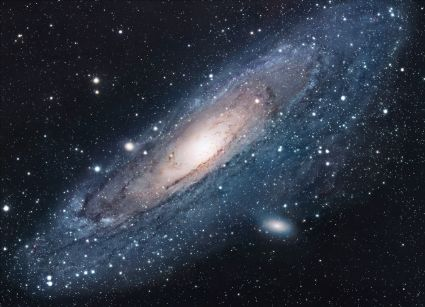
\includegraphics{universe.jpg}
		\caption{Uni 1}	
	\end{subfigure}
	\begin{subfigure}[t]{0.4\linewidth}
		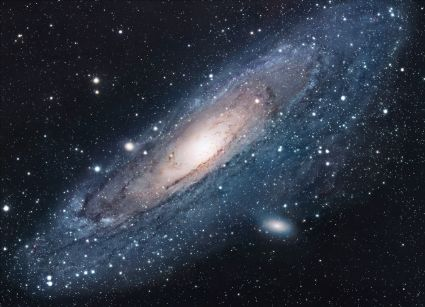
\includegraphics{universe.jpg}
		\caption{Uni 2}
	\end{subfigure}
	\begin{subfigure}[b]{\linewidth}
		\centering
		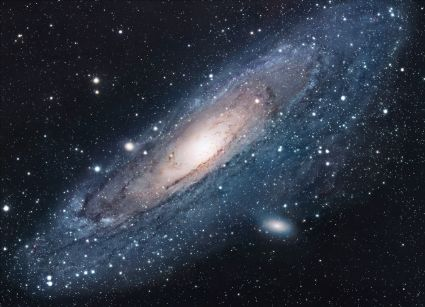
\includegraphics[width =\linewidth]{universe.jpg}
		\caption{Uni niche}
	\end{subfigure}
	\caption{Universe's}
	\label{fig:universe}
\end{figure}
\newpage
\section{Footnotes}
refer to \ref{note1}.
\footnote{\label{note1} Note1}

\newpage
\section{Table Example}

\begin{table}[h]
	\caption{Table 1}
	\centering
	\begin{tabular}{l|S|r}
		\textbf{Value 1 }& \textbf{Value 2} & \textbf{Value 3 }\\
		$\alpha$  & $\beta$ & $\gamma$ \\
		\hline
		1	&	1110.1	&	a \\
		2	&	10.1	&	b \\
		3	&	23.123131	&	c \\
	\end{tabular}
\end{table}

\section{Lists}
Itemize list with changable bullet
\begin{itemize}
	\item[--] one
	\item[$-$] two
	% From bullet to asterisk
	\item[$\ast$] three
	%Use any math character
	\item[$a$] four
	\item[--] Dash
    \item[$-$] Dash
    \item[$\ast$] Asterisk
\end{itemize}
Another itemize Example
\begin{itemize}[label=$\ast$]
    \item One
    \item Two
    \item Three
\end{itemize}

\end{document}